\documentclass[margin,line,a4paper]{resume}

\usepackage[utf8]{inputenc} %utf8
\usepackage[english,danish]{babel}
\usepackage[T1]{fontenc}
\usepackage{graphicx,wrapfig}
\usepackage{url}
\usepackage[colorlinks=true, a4paper=true, pdfstartview=FitV,
linkcolor=blue, citecolor=blue, urlcolor=blue]{hyperref}
\pdfcompresslevel=9


\begin{document}
{\sc \Large Curriculum Vitae -- Adam Jacobs}
\begin{resume}
    \vspace{0.01cm}
    \begin{wrapfigure}{R}{0.25\textwidth}
        \vspace{-1cm}
       \begin{center}
       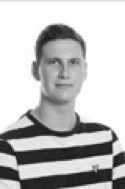
\includegraphics[width=0.15\textwidth]{adamjacobs}
       \end{center}
        \vspace{-1cm}
    \end{wrapfigure}
    
    \section{\mysidestyle Information}%\vspace{2mm}
    Adam Jacobs \\
    tel: +46704799492 \\
    email: jacobs\_feld@hotmail.com
    \href{} \\

\section{\mysidestyle Profile}\vspace{1mm}
Using optimism and curiosity to lead technological innovation. I use my experience in leading digitalization projects and hands-on knowledge of applying technology as a toolbox. Realizing amzing tech as viable business to customers make my clock tick. Currently a board member of THS (Student Union at KTH), which involves change management and decisions that affects many people.

\section{\mysidestyle Core Values}\vspace{1mm}
    \textbf{Listen}! There's always someone that knows more than you on a specific subject. Effective leadership is complementing your own skills
    \\
     \textbf{Performance!} It is achieved via effort and not how smart you are. There are no limits. If you don't know enough, then learn!
    \\
    \textbf{Courage!} Making tough decisions, standing out and being innovative takes courage. I like to spread it to others since it will then spread back to you in other ways. 

\section{\mysidestyle Education}\vspace{1mm}
    \begin{description}
        \item[KTH Computer Science] (grad. 2022)
        \item[KTH Industrial Management] (grad. 2022)
         \item[Leadership] course for children summer camps
        \item[Technology] Rudbeck Gymnasium, Sollentuna
    \end{description} 

\section{\mysidestyle Projects and Volunteering}\vspace{1mm}
\begin{description}
    \item[Jury Member] Business Model Awards 2020 
    \item[Board Member] Tekniska Högskolans Studentkår (THS) 
    \item[Team Leader] for 11 people at company Greenlytics, soft. eng. course  
     \item[System Developer] THS Armada Career Fair
    \item[App Developer] Rudbeck Gymnasium (Awarded tech project) 

\end{description}  
  
\section{\mysidestyle Work Exp.}\vspace{1mm}
\begin{description}
    \item[Intrapreneur] Ericsson ONE innovation accelerator, 
    \item[Network Engineer] Ericsson Internship, Cloud product prototype
    \item[Freelancing Consultant] Leading development of task management system for schools
    \item[Ceremony Host] at Fonus. Prepared and worked with Ceremonies. Handled grief.
    \item[Developer] educational resources app, Rudbeck Gymnasium.
    \item[Freelancing] Web developer for UF-companies
    \item[Sales] Clas Ohlson Sales Intern
\end{description}

\section{\mysidestyle References and Links}
\begin{description}
    \item[Linkedin] https://www.linkedin.com/feed/
    \item[Written] references handed in per request.
    \item[Personal Projects] https://github.com/worldyn
\end{description}

\end{resume}
\end{document} 